\section{Introduction}\label{sec:intro} 

Message passing code generation is a difficult task for an optimizing compiler targeting a distributed memory architecture. These architectures are comprised of independent units of computation called locales, each with its own set of processors, memory, and address space. For programs executed on these architectures, data is distributed across various locales of the system, and the compiler needs to reason about locality in order to determine whether a data access is remote (requiring a message to another locale to request a data element) or local (requiring no message and accessing the data element on the locale's own memory). Each remote data memory access results in a message with some non-trivial run time overhead, which can drastically slow down a program's execution time. This overhead is caused by latency on the interconnection network and locality checks for each data element. Accessing multiple remote data elements individually results in this run time overhead being incurred multiple times, whereas if they are transferred in bulk the overhead is only incurred once. Therefore, aggregating messages improves performance of message passing codes. In order to transfer remote data elements in bulk, the compiler must be sure that all elements in question are remote before the message is sent.  

The vast majority of loops in scientific programs access data using affine array accesses. An affine array access is one that is a linear expression of the loop's index variables. Loops using affine array accesses are special because they exhibit regular access patterns within a data distribution. Compilers can use this information to decide when message aggregation can take place. 

This paper presents a loop optimization for message passing code generation based on a technique called modulo unrolling. The optimization can be performed by a compiler to aggregate messages and reduce a program's execution time and communication. Modulo unrolling in its original form, pioneered by \cite{barua1999maps}, was meant to target tiled architectures such as the MIT Raw machine, not distributed memory architecutres that use message passing. It has since been modified to apply to such machines in this work. Modulo unrolling used here works by unrolling an affine loop by a factor equal to the number of locales of the machine. If the arrays used in the loop are distributed cyclically or block cyclically, each array access is guaranteed reside on a single locale across all iterations of the loop. Using this information, the compiler can then aggregate remote array accesses into a single message before and after the loop. 

We demonstrate the modulo unrolling loop optimization in practice by implementing it in Chapel. Chapel is an explicitly parallel programming language developed by Cray Inc. that falls under the Partitioned Global Address Space (PGAS) memory model. Here, a system's memory is abstracted to a single global address space regardless of the hardware architecture and is then logically divided per locale and thread of execution. By doing so, locality of reference can easily be exploited no matter how the system architecture is organized. The Chapel compiler is an open source project used by many in industry and academic settings. The language contains many high level features such as zippered iteration that greatly simplify the implementation of modulo unrolling into the language.

\subsection{Chapel's Data Distributions} 

In this work, we consider three types of data distributions: Block, Cyclic, and Block Cyclic. In a Block distribution, elements of an array are mapped to locales evenly in a dense manner. In a Cyclic distribution, elements of an array are mapped in a round-robin manner across locales. In a Block Cyclic distribution, a blocksize number of elements is allocated to consecutive array indices in a round robin fashion. Figures \ref{block_dist} - \ref{cyc_dist} illustrate these three Chapel distributions for a two-dimensional array. In Figure \ref{block_cyc_dist}, the array takes a 2 x 2 blocksize parameter. 

A programmer may choose a particular data distribution for reasons unknown to the compiler. These reasons may not even take communication behavior into account. For example, Cyclic and Block Cyclic distributions provide better load balancing of data across locales. Data redistribution may be used if elements of a data set are inserted or deleted. In particular, algorithms to redistribute data using a new blocksize exist for the Block Cyclic distribution \cite{walker1996redistribution}. If an application uses a dynamic data set with elements being appended to the end, a Cyclic or Block Cyclic distribution is superior to Block because new elements can just be added to the locale that follows the cyclic or block cyclic pattern. For Block, the entire data set would need to be redistributed every time a new element is appended. 

Allowing a data set to be compatible with other PGAS languages might be an important consideration for a programmer. If a data set is going to be used by Chapel programs and programs written in other PGAS languages, Cyclic or Block Cyclic distributions may be the best choice to distribute the data. This is because other PGAS languages, such as UPC, support Cyclic and Block Cyclic distributions but not Block. A programmer would benefit by distributing the same data set using only one scheme so the data would not have to be replicated for different programs. 

Therefore, in this work, it is our view that the compiler should not change the programmer's choice of data distribution in order to achieve better runtime and communication performance. The compiler should attempt to perform optimizations based on the data distribution that the programmer specified. 

\begin{figure}
	\begin{center}
	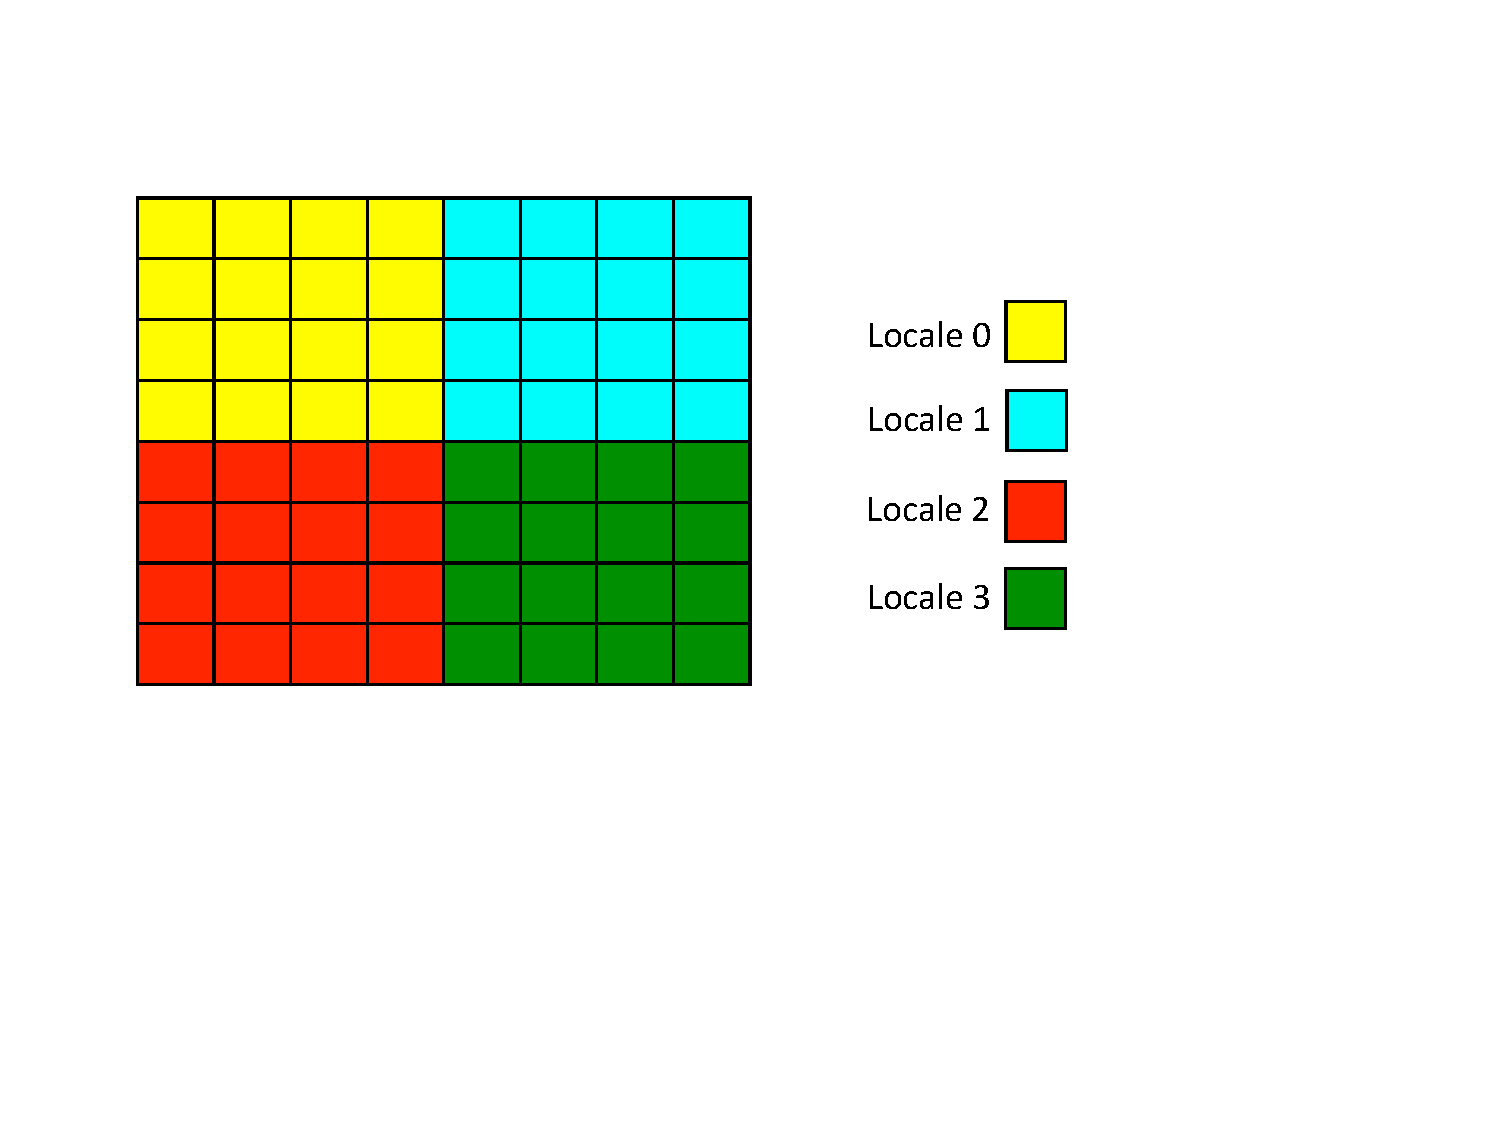
\includegraphics[scale=0.50]{./Figures/block_dist}
	\caption{Chapel Block distribution.}
	\label{block_dist}
	\end{center}
\end{figure}

\begin{figure}
	\begin{center}
	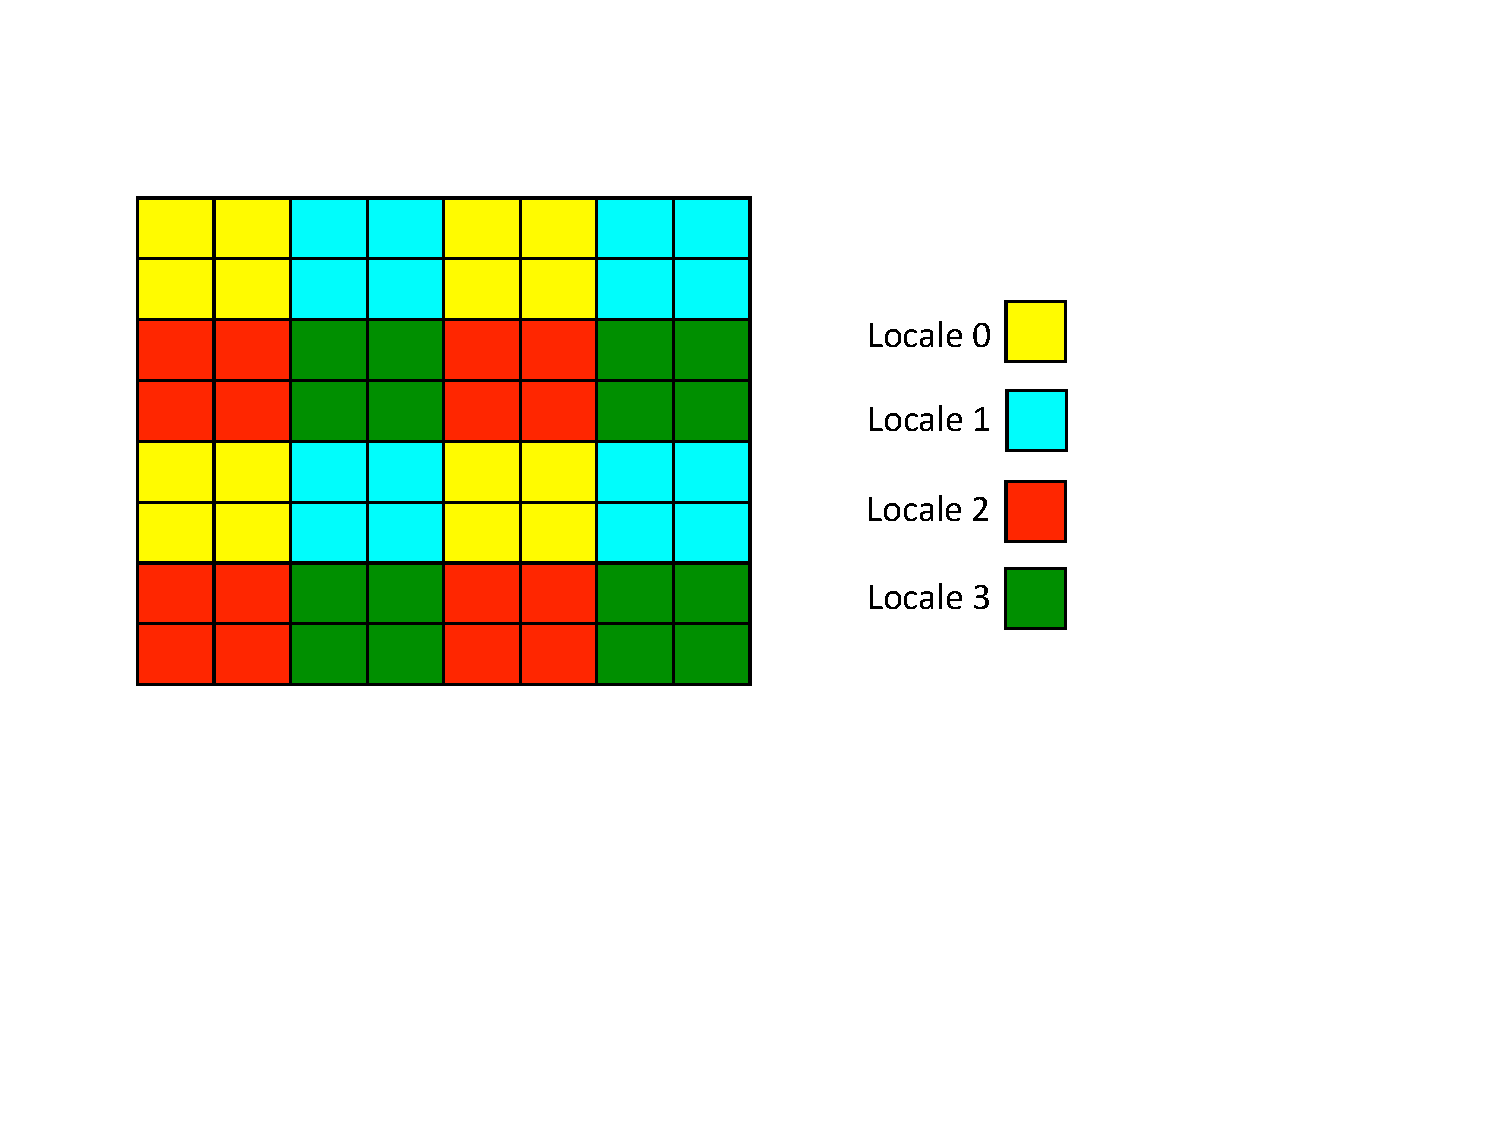
\includegraphics[scale=0.50]{./Figures/block_cyc_dist}
	\caption{Chapel Block Cyclic distribution with a 2 x 2 blocksize parameter.}
	\label{block_cyc_dist}
	\end{center}
\end{figure}

\begin{figure}
	\begin{center}
	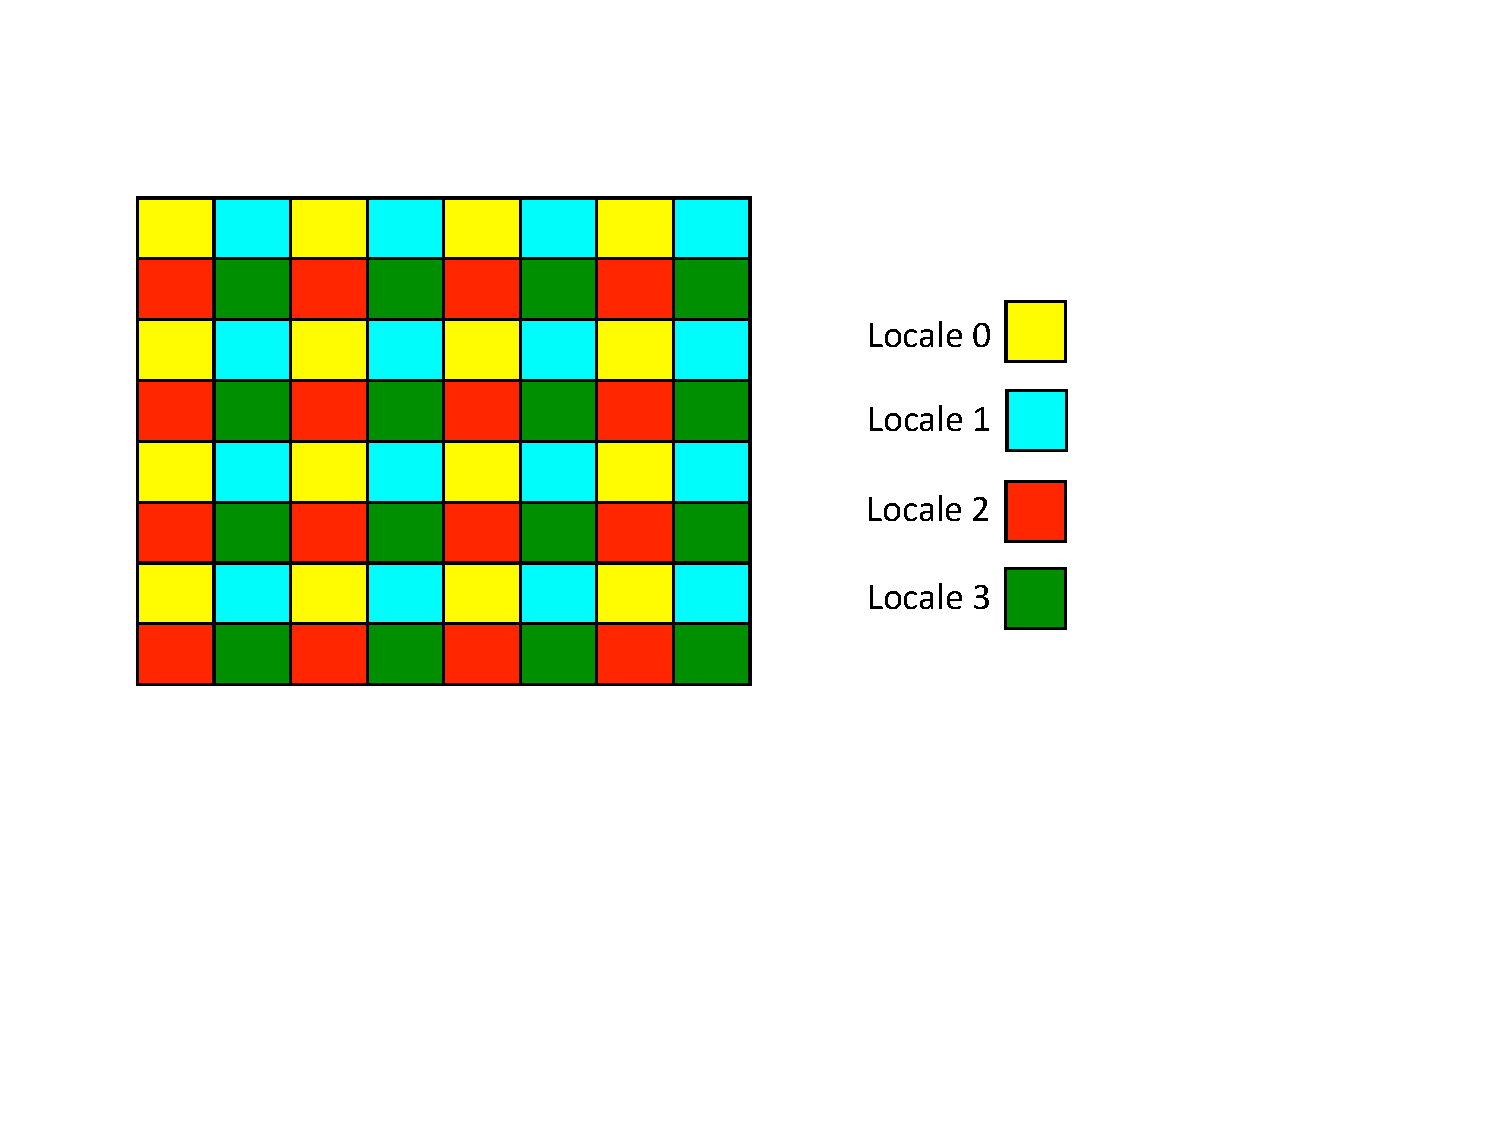
\includegraphics[scale=0.50]{./Figures/cyc_dist}
	\caption{Chapel Cyclic distribution.}
	\label{cyc_dist}
	\end{center}
\end{figure}

\begin{figure}
	\begin{center}
	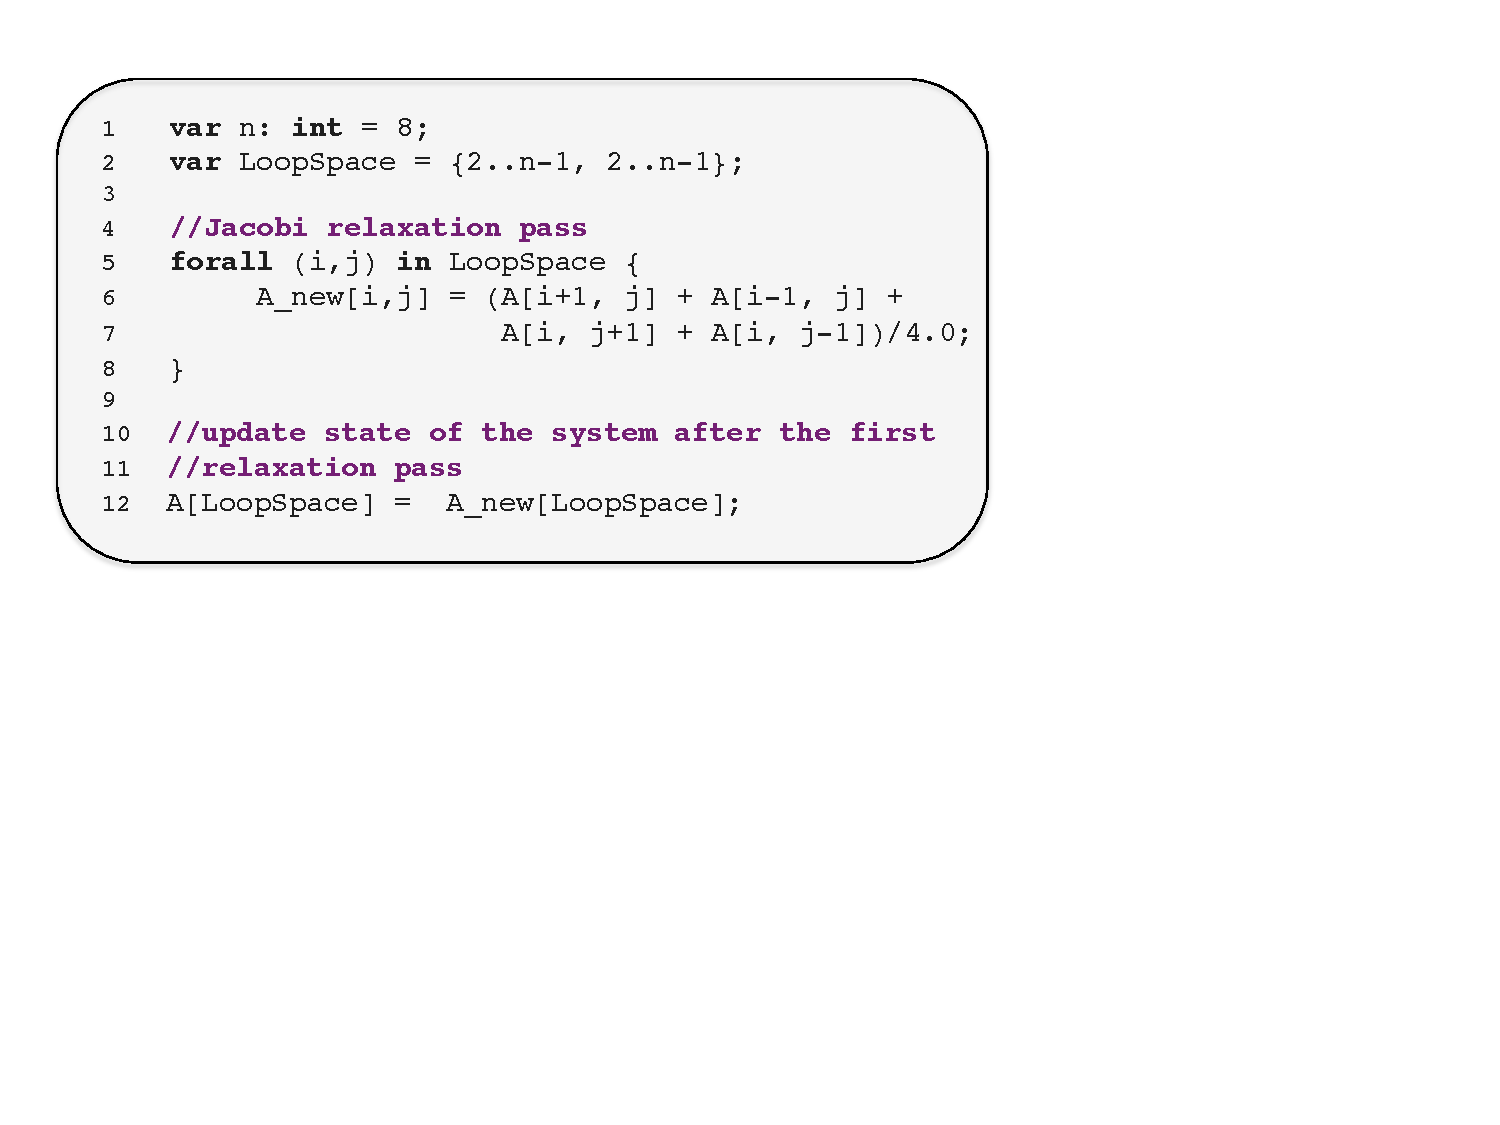
\includegraphics[scale=0.50]{./Figures/jacobi}
	\caption{Chapel code for Jacobi computation.}
	\label{jacobi_code}
	\end{center}
\end{figure}